\documentclass{article}\usepackage{knitr}

\usepackage{setspace}
\usepackage{booktabs}
\linespread{1.25}

%% Luk_pohja.tex-tiedostosta
%% Oma sivukoko
\setlength{\textheight}{9in}
\setlength{\textwidth}{6in}
\setlength{\topmargin}{0in}
%% Tekstialueen keskitys sivulle (arvot löydetty kokeilemalla)
\setlength{\oddsidemargin}{0.4cm}
\setlength{\evensidemargin}{0.4cm}

\usepackage{bm}
\usepackage{url}
\usepackage{amsmath}
\usepackage{interval}
\usepackage{setspace}
\usepackage{multirow}
\usepackage{graphicx}

\graphicspath{ {./figures/} }

\usepackage[T1]{fontenc}
\usepackage[finnish, english]{babel}
\usepackage[utf8]{inputenc}

\onehalfspacing
\usepackage[natbibapa, nodoi]{apacite}
\usepackage{tcolorbox}

\usepackage{algorithm}
\usepackage[noend]{algpseudocode}





\IfFileExists{upquote.sty}{\usepackage{upquote}}{}
\begin{document}

\thispagestyle{empty}

\thispagestyle{empty}
\begin{center}
\null\vspace{3cm}
\Large
Bayesian Inference and Adaptive Estimation in General Recognition Theory\\[2cm]
\large
Joni Pääkkö\\[1cm]
\vfill
\normalsize
\end{center}
\begin{flushright}
Maisterintutkielma\\
Jyväskylän Yliopisto\\
MUTKU\\ 
Kevät 2020
\end{flushright}

\newpage

\begin{abstract}

BACKGROUND: Bayesian adaptive estimation has been applied to many problems with good results. However not in this context, no! General Recognition Theory is a multidimensional generaliztion of Signal Detection Theory.   

Aims (which are all intertwined): 
\begin{itemize}
\item To develop General Recognition Theory by integrating it more with the theory of psychometric function.
  \begin{itemize}
  \item To argue for abandoning the ubiquitous categorization task, and to instead use a discrimination task (at least in audition)
  \item To study YesNo and 2I-4AFC tasks. 
  \end{itemize}
\end{itemize}

\begin{itemize}
\item To evaluate the widely used Bayesian adaptive procedure in the context of General Recognition Theory.
  \begin{itemize}
  \item Does it work? Are there some additional difficulties, or something to take into account? 
  \item How effective is it? How well are generating parameters recovered? How many trials are needed?
  \end{itemize}
\end{itemize}

\begin{itemize}
\item To facilitate the use of Bayesian inference in GRT. 
  \begin{itemize}
  \item Easy-to-use models are made publicly available
  \item Theory is (somewhat) developed
  \end{itemize}
\end{itemize}

METHOD: Simulation studies and psychophysical studies.

RESULTS: TBA

\end{abstract}

\newpage

\tableofcontents

\newpage

\setcounter{page}{1}
\newpage

%!Rnw root = ../Main.Rnw

\section{Simulations}

Simulations are often used in psychophysics to study the behavior of the algorithms or methods theoretically when analytical solutions are too difficult to obtain. This is the case here too. 

There are two main questions: 

\begin{enumerate}
  \item How much more efficient the adaptive algorithm is in relation to sampling stimuli from a fixed grid? 
  \item How quickly the estimates converge to generating values, and how wide the marginals of the posterior distribution are after $N$ trials?
\end{enumerate}

These questions are related, since  \textit{relative efficiency} of the algorithms (question 1) is defined here by the two other quantities: which one of the algorithms manages to more quickly gain ingormation, which is quantified by seeing how quickly the algorithms are able to minimize the marginal standard deviations of the posterior distribution. On the other hand, I'm interested in how quickly the algorithms are able to--or even if they \textit{are} able to--converge to the values of the generating parameters.

The second question has more general value: even if a method would be asymptotically unbiased and consistent\footnote{That is, bias and standard deviation go to zero as $N$ goes towards $\infty$} usually reducing bias and variance gets exponentially more costly after some point. I'm interested in estimating when this point is reached. 

\subsection{Methods}

\paragraph{Prior distributions}

Prior distributions and distributions from which generating parameters for the simulations were drawn from are shown in Figure \ref{fig:priors}. The same prior and generating distribution is used for both dimensions. Note that the scale for criterion is given in false alarm probabilities for easier interpretation. 

Priors for the parameters were chosen based on prior information from \citet{silbert2009} and from pilot testing. 

Prior for $\sigma$ was chosen to be fairly vague to reflect the possibility of widely differing thresholds.

Generating parameters for the simulations were drawn from bimodal distributions. The idea was to draw values that are covered by the prior, but which do not necessarily correspond with the mode of the prior distribution. Another motivation was to have qualitatively different simulated observers: some that have high values for some of the parameters and others that have low values.

\begin{figure}
\centering
\begin{knitrout}
\definecolor{shadecolor}{rgb}{0.969, 0.969, 0.969}\color{fgcolor}
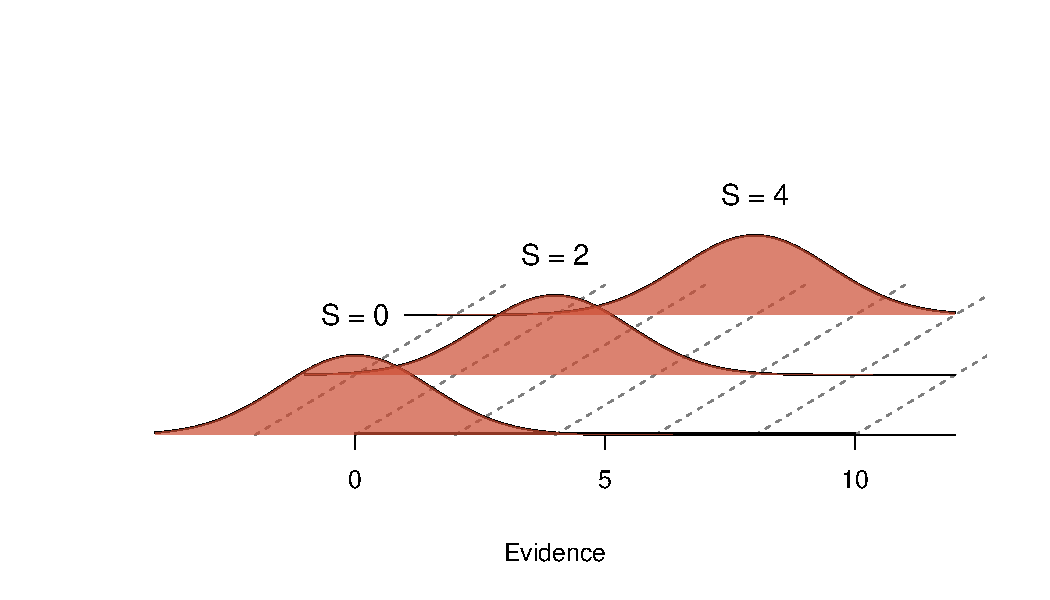
\includegraphics[width=\maxwidth]{figure/unnamed-chunk-2-1} 

\end{knitrout}

\caption{Prior distributions for the parameters of the model (solid black lines) and distributions for generating parameters for the simulations (regions shaded with red). Note that all of the densities are normalized to have maximum value of 1.0.}
\label{fig:priors}
\end{figure}

Parameters in tabular form:

\begin{table}[]
\centering
\caption{Parameters used for prior distributions and distributions of generating parameters. $M^l$ and $M^u$, respectively, are for the lower and upper peaks of bimodal distributions.}
\begin{tabular}{cccccc}
\toprule

          & \multicolumn{2}{c}{Prior} & \multicolumn{3}{c}{Generating}   \\
          \cmidrule(lr){2-3}\cmidrule(lr){4-6}
          & $M$       & $SD$    & $M^l$         & $M^u$         & $SD$   \\
\midrule
$\sigma$  & $log(2.5)$  & $0.75$   & $log(1)$    & $log(5)$    & $0.08$ \\
$C$       & $1.5$            & $0.3$   & $1.2$         & $1.7$         & $0.05$  \\
$\beta$   & $log(1)$  & $0.3$   & $log(0.8)$    & $log(1.2)$    & $0.05$ \\
$\kappa$  & $0$            & $0.3$   & $-0.25$        & $0.25$         & $0.075$ \\
$\rho$    & $0$            & $0.7$  & $atanh(0.75)$ & $atanh(-0.25)$  & $0.1$ \\
\bottomrule
\end{tabular}
\end{table}

\section{Results}


\clearpage
\bibliography{references}
\bibliographystyle{apacite}

\end{document}
